\section{Data}
\label{sec:meth}


\subsection{Description of the data}
Data verzameling en beschrijving van de data jajaja

Hoe is de data verzameld, en hoe heb jij die data verkregen?


Wat staat er in de data? Niet alleen maar een technisch verhaal, maar ook inhoudelijk. DE lezer moet een goed idee krijgen over de technische inhoud en wat het betekent.

\pagebreak
\subsection{Wat plotjes en tabelletjes}

Zie het IPython Notebook \url{PandasAndLatex.ipynb} voor de code om vanuit pandas een poltje op te slaan en een dataframe als tabel op te slaan. Het werkt ideaal! 

De interrupties van Wilders staan beschreven in Figure~\ref{fig:wilders} en Tabel~~\ref{tab:Wilders}.


\begin{figure}
\begin{center}
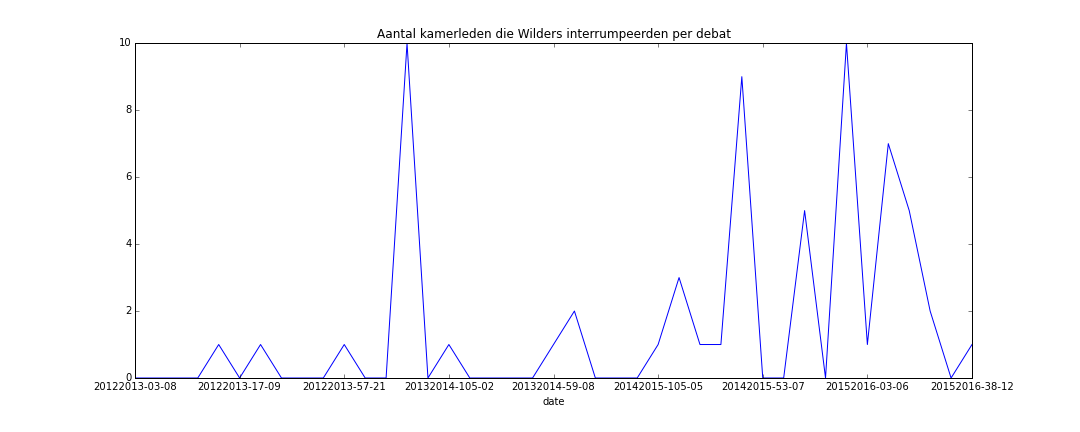
\includegraphics[width=\linewidth]{WildersPlot.png}
\caption{\label{fig:wilders} Aantal interrupties van Wilders in de Tweede Kamer door de tijd (periode 2012-2016).}
\end{center}
\end{figure}


\pagebreak

\begin{table}[h]
\begin{footnotesize}
\begin{tabular}{lrl}
\toprule
{} &  indegree &                               interruptie\_volgorde \\
date            &           &                                                    \\
\midrule
20122013-03-08  &         0 &                                                    \\
20122013-07-16  &         0 &                                                    \\
20122013-100-03 &         0 &                                                    \\
20122013-100-06 &         0 &                                                    \\
20122013-17-06  &         1 &                         Pechtold-Pechtold-Pechtold \\
20122013-17-09  &         0 &                                                    \\
20122013-21-04  &         1 &                         Pechtold-Pechtold-Pechtold \\
20122013-22-08  &         0 &                                                    \\
20122013-32-06  &         0 &                                                    \\
20122013-48-23  &         0 &                                                    \\
20122013-57-21  &         1 &  Pechtold-Pechtold-Pechtold-Pechtold-Pechtold-P... \\
20122013-76-03  &         0 &                                                    \\
20122013-76-06  &         0 &                                                    \\
20132014-05-02  &        10 &  Roemer-Roemer-Van Haersma Buma-Van Haersma Bum... \\
20132014-06-04  &         0 &                                                    \\
20132014-105-02 &         1 &  Pechtold-Pechtold-Pechtold-Pechtold-Pechtold-P... \\
20132014-105-06 &         0 &                                                    \\
20132014-14-03  &         0 &                                                    \\
20132014-14-06  &         0 &                                                    \\
20132014-52-18  &         0 &                                                    \\
20132014-59-08  &         1 &                               Klaver-Klaver-Klaver \\
20142015-02-08  &         2 &  Pechtold-Pechtold-Pechtold-Pechtold-Pechtold-P... \\
20142015-03-06  &         0 &                                                    \\
20142015-09-09  &         0 &                                                    \\
20142015-100-05 &         0 &                                                    \\
20142015-105-05 &         1 &                                  Pechtold-Pechtold \\
20142015-111-04 &         3 &  Pechtold-Pechtold-Pechtold-Pechtold-Pechtold-P... \\
20142015-111-07 &         1 &                                  Pechtold-Pechtold \\
20142015-39-71  &         1 &                                  Pechtold-Pechtold \\
20142015-41-07  &         9 &  Samsom-Samsom-Pechtold-Pechtold-Pechtold-Kuzu-... \\
20142015-53-07  &         0 &                                                    \\
20142015-61-23  &         0 &                                                    \\
20142015-79-07  &         5 &  Klaver-Klaver-Klaver-Gesthuizen-Gesthuizen-Ges... \\
20142015-95-06  &         0 &                                                    \\
20152016-02-07  &        10 &  Pechtold-Pechtold-Pechtold-Pechtold-Slob-Slob-... \\
20152016-03-06  &         1 &       Pechtold-Pechtold-Pechtold-Pechtold-Pechtold \\
20152016-14-02  &         7 &  Klaver-Klaver-Roemer-Roemer-Roemer-Roemer-Sams... \\
20152016-14-05  &         5 &  Van Haersma Buma-Van Haersma Buma-Van Haersma ... \\
20152016-27-03  &         2 &  Segers-Segers-Segers-Segers-Kuzu-Kuzu-Kuzu-Kuz... \\
20152016-38-10  &         0 &                                                    \\
20152016-38-12  &         1 &                                        Klein-Klein \\
\bottomrule
\end{tabular}

\end{footnotesize}
\caption{\label{tab:Wilders} Door wie werd Wilders onderbroken en hoe vaak per debat.}
\end{table}


\pagebreak
\subsection{Methods}
Hoe je je vraag gaat beantwoorden.


Dit is de langste sectie van je scriptie. 

Als iets erg technisch wordt kan je een deel naar de Appendix verplaatsen. 

Probeer er een lopend verhaal van te maken.

Het is heel handig dit ook weer op te delen nav je deelvragen:

\subsubsection{RQ1}

\subsubsection{RQ2}